\section{Implementación del protocolo IoTorii}
\label{sec:devIOTTORIII}

En esta sección se va a explicar la implementación realizada del protocolo IoTorii en el \textit{software switch} \gls{bofus}. Dado que el trabajo de implementación ha sido bastante extenso, dado que había que discernir que parte de la implementación del control in-band podía ser aprovechada, se ha decidido generar un documento anexo \cite{davidBOFUSS} aparte de la memoria, donde se explique a bajo nivel las modificaciones realizadas. Todo el código se puede encontrar indicado en la Sección \ref{sec:estadoArte_github}. \\
\\
En la Figura \ref{fig:WIN-BOFUSS}, se puede apreciar la secuencia lógica que se ha llevado a cabo para la implementación del protocolo IoTorii en el software switch. En adelante se podrá encontrar el termino \texttt{win-BOFUSS}, el cual hará referencia a la implementación del protocolo IoTorii en la implementación de in-band del \gls{bofus}, conocida como \texttt{in-BOFUSS}, por lo que para añadirle la condición de \textit{wireless} se ha apodado como \texttt{win-BOFUSS}, del inglés \textit{\textbf{w}ireless \textbf{in}-band \textbf{B}asic \textbf{O}pen\textbf{F}low \textbf{U}serspace \textbf{S}oftware \textbf{S}witch}.\\

% fig
\begin{figure}[ht!]
    \centering
    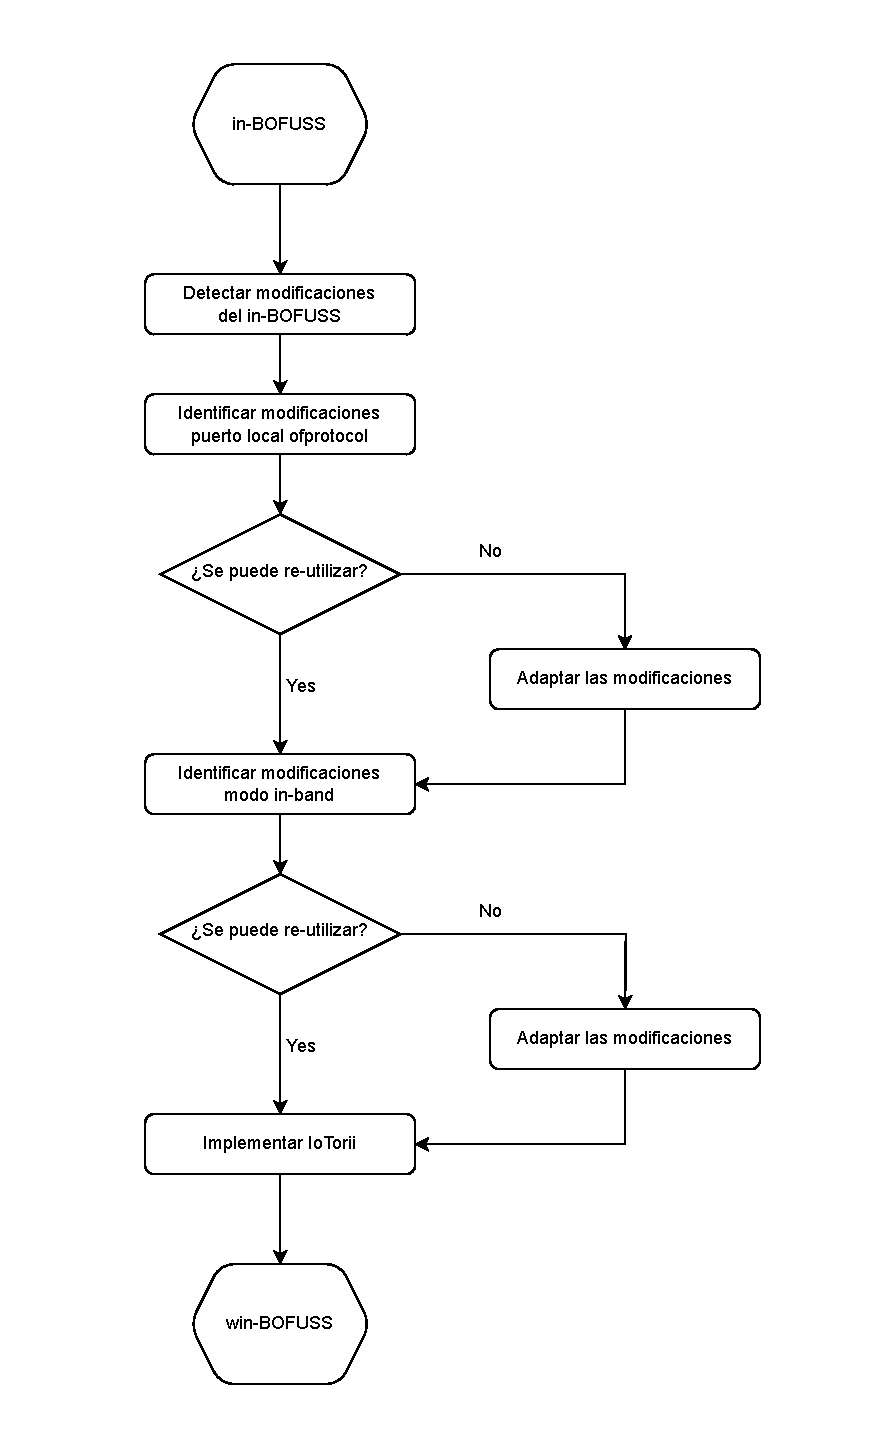
\includegraphics[width=0.75\textwidth]{archivos/img/dev/winBOFUSS.pdf}
    \caption{Diagrama de flujo para la implementación del protocolo IoTorii en el software switch \glsentryshort{bofus}}
    \label{fig:WIN-BOFUSS}
\end{figure}

La implementación de IoTorii está basada en una publicación del grupo de investigación NetIS de la Universidad de Alcalá \cite{rojas2021outperforming}. El funcionamiento del protocolo está descrito en la Sección \ref{sec:ana_inband}, y con él conseguiremos crear múltiples caminos desde cualquier nodo de la topología al nodo raíz. La idea de utilizar este protocolo según se comentó es para tener caminos de respaldo en cada nodo hacia el nodo raíz, pudiendo conmutar de uno a otro cuando sea necesario, bien sea porque un equipo ha fallado o porque al ser un entorno inalámbrico donde la movilidad es intrinseca el \textit{next-hop} al nodo raíz ya no se encuentra en rango.\\
\\
En la Figura \ref{fig:iotoriiFulls}, se indica el diagrama de flujo con la implementación del protocolo en el \gls{bofus}. En primer lugar, al poner el switch en el modo de control in-band, se inicializa la lógica de IoTorii. Una vez que el protocolo IoTorii ha sido inicializado, el nodo raíz comienza la exploración, propagando los paquetes utilizados para generar los caminos que posteriormente serán almacenados en las tablas IoTorii de los nodos. Dichos paquetes, de tipo \textit{SetHLMAC}, solo serán entregados a los nodos que cumplan la condición de vecinos, es decir, aquellos nodos que hayan sido notificados mediante un mensaje de tipo \textit{Hello}. Cuando una ruta de la tabla HLMAC no se ve renovada, es decir, el nodo anexo al siguiente salto de esa ruta no ha enviado un mensaje de tipo \textit{Hello}, esta ruta se invalidará y se saltará a la siguiente dentro de la tabla HLMAC. Cuando esto ocurre el puerto local será el mismo, dado que la interfaz será la misma, pero el \textit{next-hop} no lo será dado que cambiará, habrá que actulizar la MAC destino en la conexión TCP que se realiza através de un mensaje netlink al stack de red del Kernel. \\
\\
En un entorno Linux, es posible utilizar Netlink para modificar la dirección MAC de destino asociada a una IP específica en la tabla ARP. Netlink es una interfaz de comunicación entre el espacio de usuario y el espacio de Kernel que permite realizar diversas operaciones relacionadas con la configuración de red. Lo primero que se tiene que llevar a cado en esta operación es abrir una conexión Netlink para comunicarse con el Kernel. Esto implica crear un socket Netlink y enlazarlo a un tipo de mensaje Netlink en específico. Acto seguido, se tiene que preparar el mensaje Netlink de tipo \texttt{RTM\_NEWNEIGH} (mensaje utilizado para manipular la caché ARP), y establecer los atributos del mensaje, configurando los atributos del mensaje para indicar la IP y la nueva dirección MAC destino a fijar. Enviar dicho mensaje y gestionar la confirmación del Kernel. De esta forma podremos actualizar de una ruta HLMAC a otra, pero lamentablemente no se ha conseguido hacer la operación de forma automática sin cerrar el socket por lo que será necesario volver a abrir el socket TCP con el controlador.\\
\\



\begin{figure}[ht!]
    \centering
    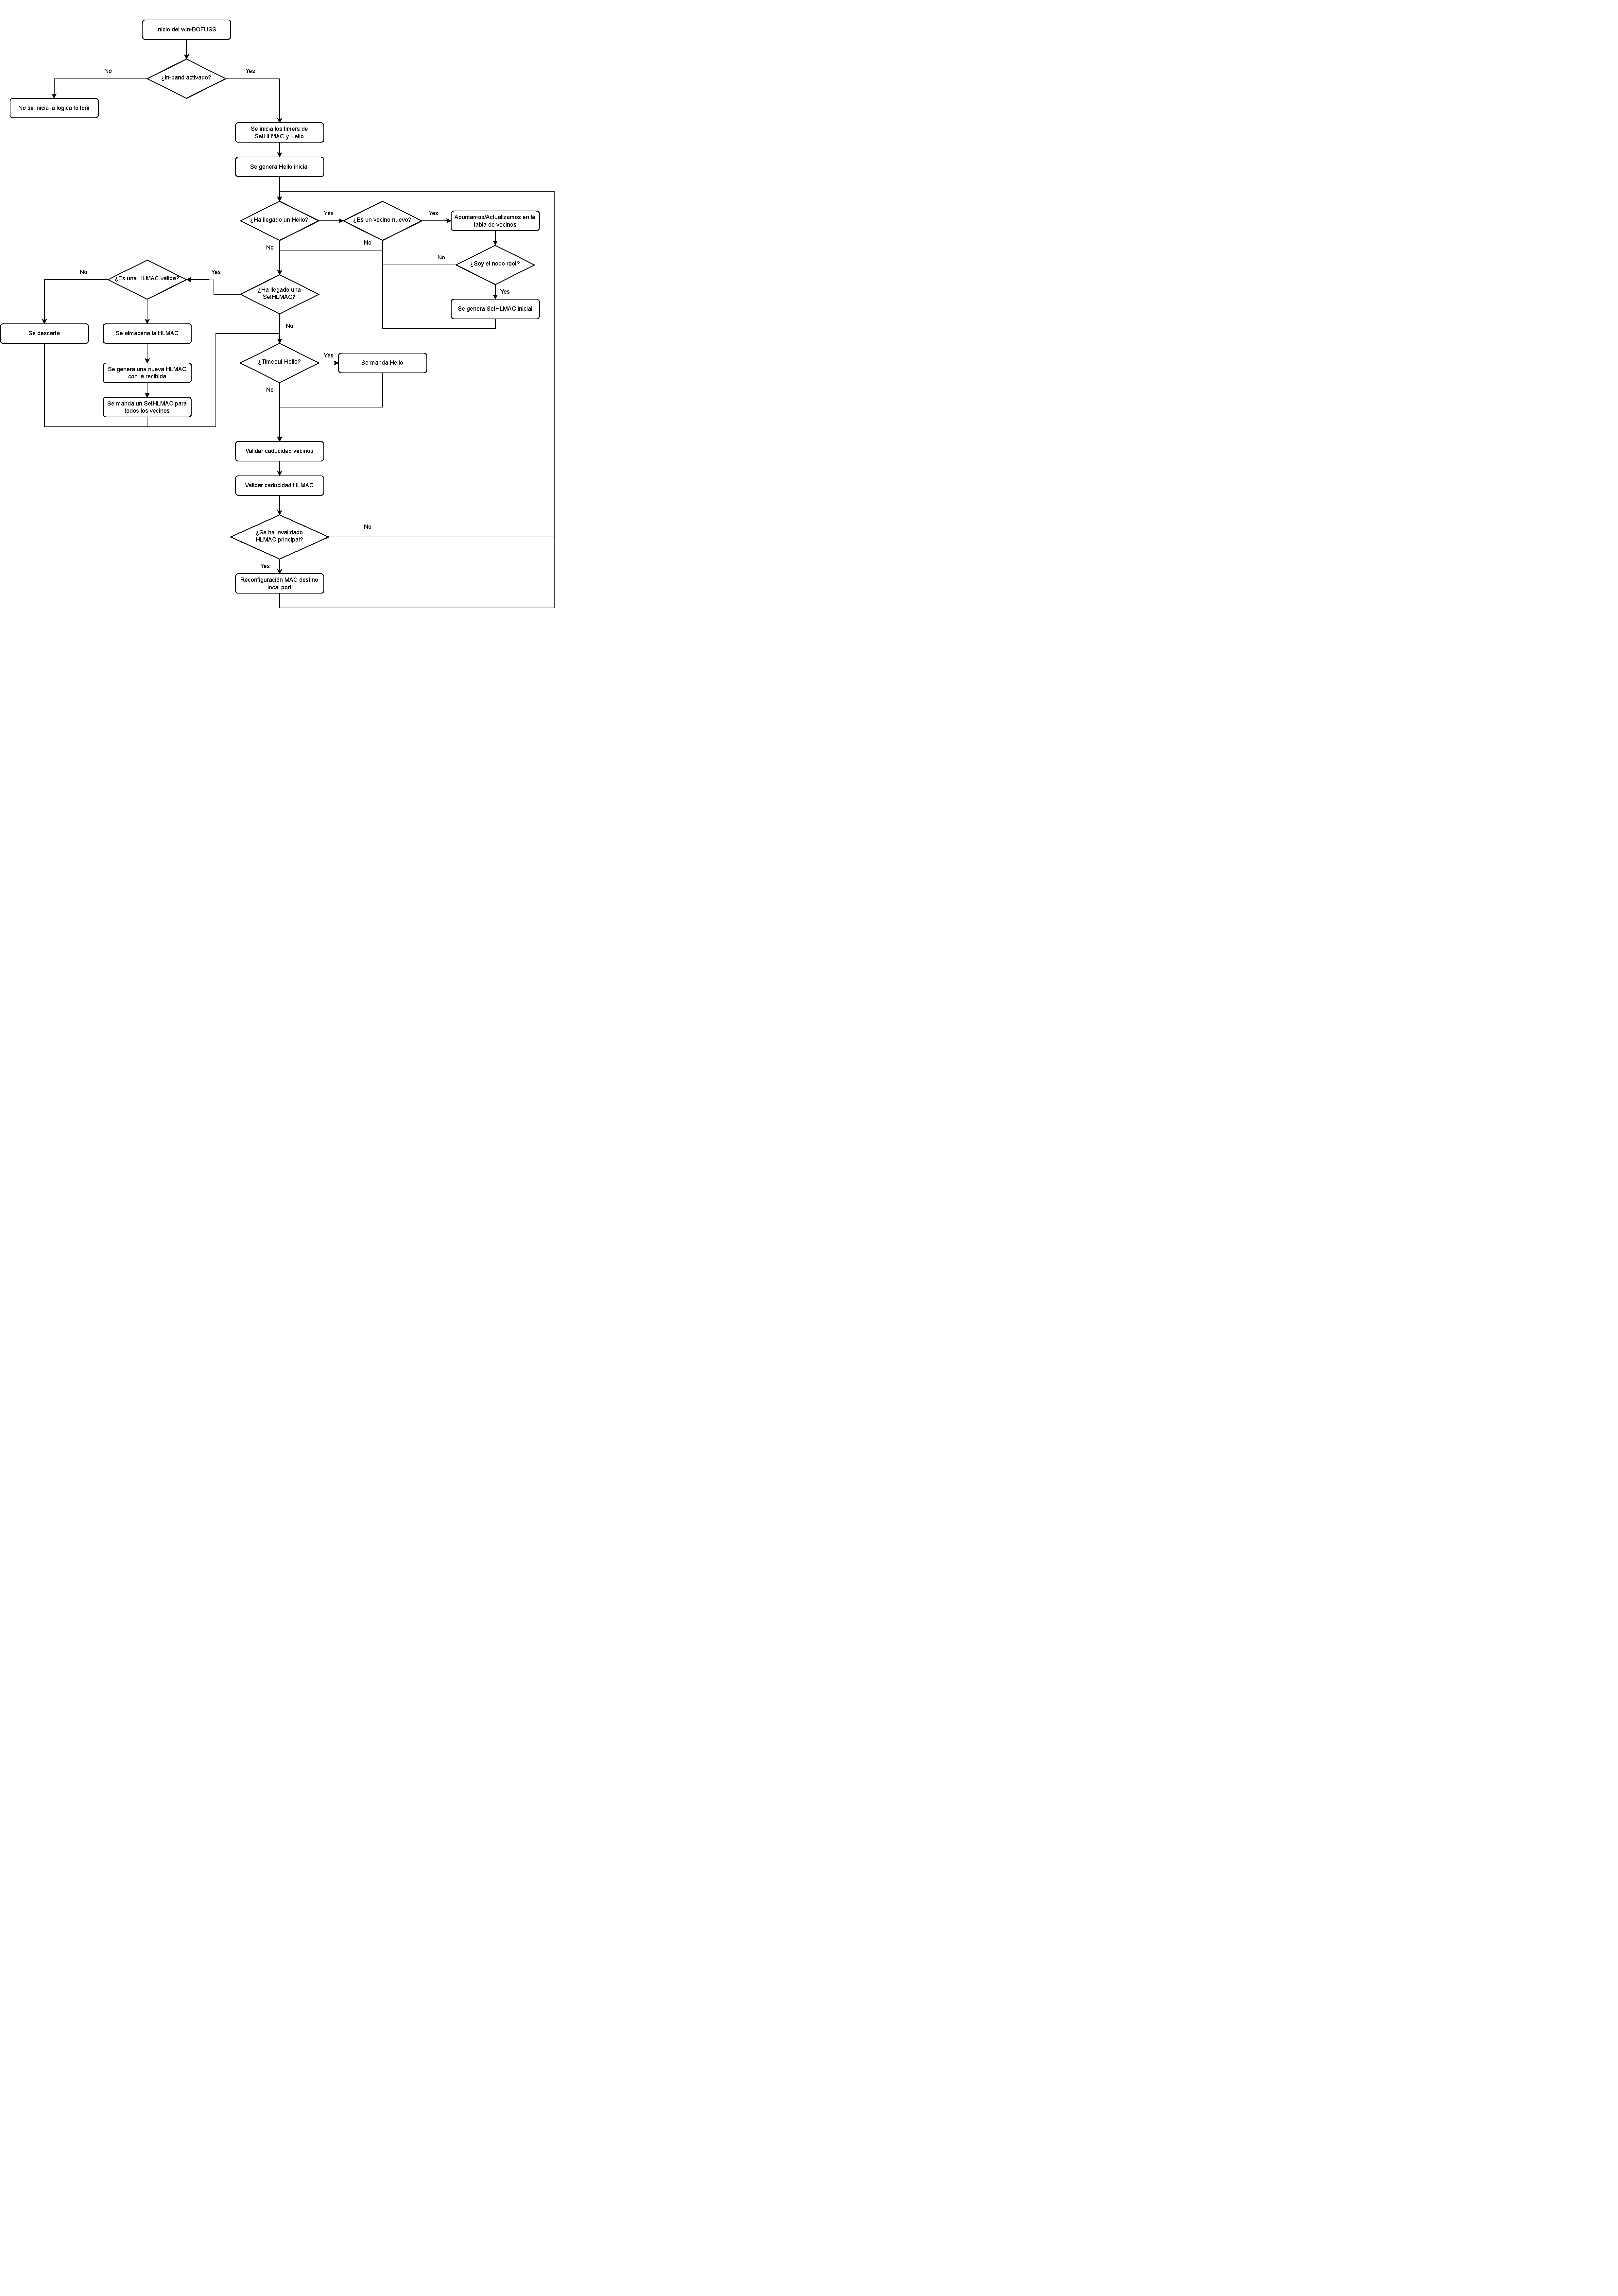
\includegraphics[width=\textwidth]{archivos/img/dev/iotorii.pdf}
    \caption{Diagrama de flujo de la operativa del protocolo IoTorii en el software switch \glsentryshort{bofus}}
    \label{fig:iotoriiFulls}
\end{figure}

\newpage

La importancia de establecer un temporizador para los mensajes \textit{Hello} y definir la caducidad de los vecinos en un protocolo radica en la mejora de su resiliencia y capacidad para adaptarse a cambios en la topología de la red. Estos mecanismos son fundamentales para mantener la conectividad y la estabilidad del protocolo en entornos dinámicos.\\
\\
El temporizador de los mensajes \textit{Hello} determina la frecuencia con la que los nodos del protocolo intercambian información de vecindad. Estos mensajes \textit{Hello} son vitales para conocer y mantener actualizada la lista de vecinos en la red. Al establecer un temporizador adecuado, se asegura que los nodos compartan regularmente información sobre su disponibilidad, estado y conexiones. Esto permite identificar rápidamente cambios en la topología de la red, como la caída de un enlace o la aparición de nuevos nodos. La caducidad de los vecinos define el tiempo que un nodo considera que un vecino sigue siendo alcanzable y activo. Cuando un vecino no responde a los mensajes \textit{Hello} dentro de este período, se considera que ha caducado y se elimina de la lista de vecinos. Establecer una caducidad adecuada es esencial para detectar y reaccionar rápidamente ante la pérdida de conectividad con un vecino. Al eliminar los vecinos caducados, se evita enviar tráfico a nodos inalcanzables y se garantiza que los recursos de red se utilicen de manera eficiente.\\
\\
La resilencia de un protocolo depende en gran medida de su capacidad para recuperarse rápidamente de fallos en la red y adaptarse a cambios en la topología. Al establecer un temporizador de mensajes \textit{Hello} y una caducidad de vecinos adecuados, el protocolo puede detectar y responder de manera oportuna a eventos como enlaces caídos, nodos inalcanzables o nuevos vecinos. Esto permite que el protocolo reconstruya rápidamente su tabla de vecinos y ajuste sus rutas en consecuencia, minimizando el impacto de las fallos y optimizando la utilización de los recursos de red.\\
\\
A continuación se van a indicar algunas de las modificaciones más importantes a la hora de implementar la lógica del protocolo IoTorii.

\begin{itemize}
    \item La estructura \texttt{reg\_HLMAC}, ha sido creada para representar una entrada de la tabla de HLMACs, también conocida como tabla de rutas de IoTorii. Cada entrada tiene almacenada la HLMAC, un flag de si está activa o no.
    \item La estructura \texttt{table\_HLMAC}, ha sido creada para representar la tabla de HLMACs, que viene a ser una lista enlazada simple de estructuras \texttt{reg\_HLMAC}.
    \item La estructura \texttt{reg\_nb}, ha sido creada para representar una entrada de la tabla de vecinos. Cada entrada tiene almacenada la MAC real del vecino, un flag de si está activa o no, y el sufijo único asignado.
    \item La estructura \texttt{table\_nb}, ha sido creada para representar la tabla de vecinos, que viene a ser también una lista enlazada simple de estructuras \texttt{reg\_nb}.
    \item Se ha adaptado la función \texttt{table\_AMACS\_add\_AMAC()} con las nuevas estructuras de datos, para que gestione el guardado de las HLMACs de IoTorii en vez de las AMACs. La función se ha renombrado a \texttt{table\_HLMACS\_add\_HLMAC()}.
    \item Se ha modificado la función \texttt{dp\_ports\_output\_amaru()}, la cual se encargaba de crear y enviar un paquete de Amaru por todas las interfaces del switch, para que ahora, dado que solo va a haber una interfaz genere los mensajes \textit{SetHLMAC} por la interfaz por los $N$ vecinos que tenga el nodo en cuestión. La función se ha renombrado a \texttt{dp\_ports\_output\_iotorii()}.
    \item Se han adaptado las funciones \texttt{disable\_invalid\_amacs\_UAH()} y \texttt{enable\_valid\_\\amacs\_UAH()}, las cuales se utilizaban para conmutar el \textit{flag} de active de las rutas, para que puedan trabajar con las nuevas estructuras de datos HLMAC. Las funciones se han renombrado a \texttt{disable\_invalid\_hlmacs\_UAH()} y \texttt{enable\_valid\_hlmacs\_UAH()} respectivamente.
    \item Se ha modificado la función \texttt{configure\_new\_local\_port\_amaru\_UAH()}, la cual se encargaba de buscar en la tabla de rutas AMACS, para que busque en la nueva tabla HLMAC y que aparte gestione el traspaso de una ruta a otra, modificando vía Netlink la nueva MAC destino del siguiente salto. La función se ha renombrado a \texttt{configure\_new\_local\_port\_iotorii\_UAH()}.
    \item Se ha modificado la función \texttt{send\_amaru\_new\_localport\_packet\_UAH()}, para que ajuste las reglas de las tablas de flujos del ofdatapath mediante una generación de un mensaje de tipo \texttt{PACKET\_IN} que se envía al ofprotocol.
    \item Se ha modificado la función \texttt{dp\_ports\_run()}, la cual de forma periorida verificará el estado del puerto, y además gestionará las funciones \texttt{disable\_invalid\_amacs\_UAH()} y \texttt{enable\_valid\_amacs\_UAH()} verificando la caducidad de las entradas. En caso de caducar una ruta activa se llamará a la función, \texttt{install\_new\_localport\_rules\_UAH()}, y a la función \texttt{configure\_new\_local\_port\_iotorii\_UAH()} para gestionar la instalación de una ruta alternativa.
    \item Se han creado una lógica de control de timer para la generación de los mensajes \textit{Hello}s. Toda la lógica está incluida en la función \texttt{timer\_UAH()}.
\end{itemize}

\subsection{Despliegue de la implementación en una RPi}

Durante el proceso de desarrollo, se ha realizado un intento exhaustivo para desplegar la implementación completa del protocolo IoTorii en una Raspberry Pi (RPi). Sin embargo, hasta el momento, este intento no ha alcanzado el éxito debido a una problemática relacionada con la traducción de símbolos que se realiza en la librería de \texttt{oflib}. Se ha identificado que esta traducción debe ser corregida para lograr un despliegue funcional en dicha plataforma, pero se escapa de los objetivos del \gls{tfm}. Por otro lado, se ha observado que el despliegue del \gls{bofus}, una vez se ha corregido el funcionamiento interno de la librería en cuestión, debería ser inmediato, ya que el entorno Linux es el mismo, y solo se requiere adaptarse correctamente a la arquitectura. Es relevante mencionar que se ha identificado un \textit{issue} específico que refleja esta misma problemática de despliegue sobre una arquitectura ARM, la misma que se ha visto a la hora de desplegar la implementación del protocolo IoTorii.

\begin{itemize}
    \item Dicho \textit{issue}  puede consultarse en el siguiente enlace: \url{https://github.com/CPqD/ofsoftswitch13/issues/196}
\end{itemize}

